\documentclass{article}



\usepackage{arxiv}

\usepackage[utf8]{inputenc} % allow utf-8 input
\usepackage[T1]{fontenc}    % use 8-bit T1 fonts
\usepackage{hyperref}       % hyperlinks
\usepackage{url}            % simple URL typesetting
\usepackage{booktabs}       % professional-quality tables
\usepackage{amsfonts}       % blackboard math symbols
\usepackage{nicefrac}       % compact symbols for 1/2, etc.
\usepackage{microtype}      % microtypography
\usepackage{lipsum}		% Can be removed after putting your text content
\usepackage{graphicx}
\usepackage{natbib}
\usepackage{doi}
\usepackage{amsmath}
\usepackage{amsthm}
\usepackage{tikz}
\usepackage{pgfplots}
\usepackage{todonotes}
\usetikzlibrary{patterns}
\usepgfplotslibrary{fillbetween}
\pgfplotsset{compat=1.17}
\newtheorem{theorem}{Theorem}
\newtheorem{proposition}{Proposition}


\title{Multidimensional Extension of Buffon's Needle Problem}

%\date{September 9, 1985}	% Here you can change the date presented in the paper title
%\date{} 					% Or removing it

\author{ Alexander~Choi\\
	alexander.e.choi@gmail.com
}

% Uncomment to remove the date
%\date{}

% Uncomment to override  the `A preprint' in the header
%\renewcommand{\headeright}{Technical Report}
%\renewcommand{\undertitle}{Technical Report}
\renewcommand{\shorttitle}{Multidimensional Buffon's Needle}

%%% Add PDF metadata to help others organize their library
%%% Once the PDF is generated, you can check the metadata with
%%% $ pdfinfo template.pdf
\hypersetup{
pdftitle={Multidimensional Extension of Buffon's Needle Problem},
pdfsubject={q-bio.NC, q-bio.QM},
pdfauthor={Alexander E.~Choi},
pdfkeywords={Buffon's needle problem, Geometric probability},
}

\begin{document}
\todo{Get rid of all "we". I'm a bit conflicted on whether it's supposed to be active or passive voice, but most seem to be passive?}
\maketitle

\begin{abstract}
	Consider a line segment randomly placed on a two-dimensional plane ruled with a set of regularly spaced parallel lines. The classical Buffon's needle problem
    asks what the probability is that the line segment intersects at least 1 of these lines. This paper extends this problem by considering a line segment randomly
    placed in $\mathbb{R}^D$ and its probability of intersection with a set of regularly spaced parallel hyperplanes. 
\end{abstract}


% keywords can be removed
\keywords{Buffon's needle problem \and Geometric Probability}

\section{Introduction}
Buffon's needle problem was originally posed in the 18th century with the following premise. Given a line segment, or "needle", of length $r$ randomly dropped on a two-dimensional plane
ruled with a set of parallel lines regularly spaced $s$ units apart, what is the probability that the needle crosses at least 1 of the lines? The solution, it turns out, is
$\frac{2r}{s\pi}$ when $r<s$. Variations and extensions of this problem have been investigated as well, including
\begin{itemize}
	\item Laplace's Extension - Investigating when the plane is gridded with 2 orthogonal sets of parallel lines with spacings $s_1$ and $s_2$.
	\item Buffon's Noodle - Instead of being rigidly straight, the needle is permitted to bend (a "noodle").
	\item Pivot Needle - The needle is constructed of two line segments that hinge together. Each crossing is considered.
\end{itemize}

In this paper, we investigate a particular extension that allows the needle to be dropped into a space with dimension greater than 2. In these higher dimensions, we will rule the space
with parallel hyperplanes rather than lines. Additionally, we will look at gridding the space with orthogonal sets of hyperplanes, thereby extending Laplace's extension into higher dimensions.

Given $D\in\mathbb{N}_{>0}$ and $N\in[1,2,\dots,D]$, consider a grid on $\mathbb{R}^D$ formed by $N$ orthogonal sets of regularly spaced hyperplanes where each set of hyperplanes
has a potentially unique spacing of $S_i$. For example, if $D=2, N=1, S_1=2$, the grid would match the original Buffon Needle problem and would have only a single set of parallel lines 2 units apart.
If $D=2, N=2, S=[1, 2]$, the grid would have 2 sets of parallel lines that are orthogonal to each other, matching the problem in Laplace's extension. One set of lines would have a spacing of 1 unit and 
the other would have a spacing of 2 units.
\missingfigure[]{Depictions of the buffon needle and laplace extension}
\begin{tikzpicture}
	
\end{tikzpicture}

A line segment of length $r\in\mathbb{R}^+$ is randomly located in the space such that one of its end points, $P_0$, is uniformly distributed
across the entire domain. The line segment's orientation is independently distributed such that when considering $P_0$ as the center of a $(D-1)$-sphere of radius $r$, the other point, $P_1$,
is uniformly distributed on the surface of that hypersphere. This line segment may intersect with $C\in\mathbb{N}$ unique hyperplanes. This paper studies the probability that the line segment
intersects with at least $c$ hyperplanes, $P(C\ge c|r, D, N, S)$. From there, solutions for crossing less than $c$ hyperplanes and exactly $c$ hyperplanes can
be derived.

We will define the coordinates of line segment using $\vec{x}\in\mathbb{R}^D$ for the location of $P_0$ and spherical coordinates for the location of $P_1$ with respect to $P_0$.

\begin{align*}
    y_1 &= r\cos{\phi_1}\\
    y_2 &= r\sin{\phi_1}\cos{\phi_2}\\
    \vdots\\
    y_{D-1} &= r\sin{\phi_1}\hdots\sin{\phi_{D-2}}\cos{\phi_{D-1}}\\
    y_{D} &= r\sin{\phi_1}\hdots\sin{\phi_{D-2}}\sin{\phi_{D-1}}\\
    P_1 &= \vec{x} + \vec{y}\\
	\phi_j &\in \begin{cases}[0, \pi] & j<D-1 \\ [0, 2\pi] & j=D-1\end{cases}
\end{align*}

Translational symmetry of the grid of hyperplanes allows us to consider the domain of $P_0$ to be $x_i\in[0,S_i]$ as the origin can be moved to any point on the grid.
Reflectional symmetry of the grid also allows us to consider the domain of $\vec{y}$ to be a single orthant of the hypersphere. For convenience, we will pick the orthant where
$\phi_i \in [0, \pi/2]$.

The rest of the paper is organized as follows. A derivation of the joint probability density function for $P_0$ and $P_1$ will be provided in \S 2. The derivation and validation
of the crossing probabilities for $N=1$ will be given in \S 3. The derivation and validation of the crossing probabiities for any $N$ and $r<\min(S)$ will be given in \S 4. Analysis of the limits
and extrema of the probabilities is explored in \S 4.

\section{Joint Probability Density of the Line Segment}
Each coordinate for $P_0$ can be defined as a uniformly distributed random variable $X_i\sim{\rm Uniform}(0,S_i)$. Due to independence, the joint PDF for $P_0$ is the product
$\prod_{i=1}^D \frac{1}{S_i}$. By the definition of the problem, the coordinates $\vec{x}$ do not influence the orientation of the line segment defined by $\vec{\phi}$. 
The probability density function for the uniform distribution of points on an orthant of the hypersphere can be determined by calculating the area element in terms of spherical coordinates.

\begin{proposition}
In spherical coordinates, the probability density function for a uniform distribution on an orthant of a hypersphere is $\frac{2^D}{A_{D-1}}\prod_{j=1}^{D-1}r\sin^{D-1-j}\phi_j$ where
$A_{D-1}$ is the surface area of a $(D-1)$-sphere.
\end{proposition}
\begin{proof}
	The area element of an $(D-1)$-sphere of radius $r$ can be expressed as 
	\begin{equation} \label{eq:1}
	d\Omega = \left(\prod_{j=1}^{D-1}r\sin^{D-1-j}\phi_j\right)d\phi_1 \hdots d\phi_{D-1}
	\end{equation}
	The probability that a point lies in this differential element can be expressed as follows.
	\begin{equation} \label{eq:2}
	f_{\Omega}(\Omega)d\Omega = f_{\vec{\phi}}(\phi_1, \hdots, \phi_{D-1})d\phi_1 \hdots d\phi_{D-1}
	\end{equation}
	The points are uniformly distributed over the surface of an orthant of the hypersphere implying that $f_{\Omega}(\Omega) = \frac{2^D}{A_{D-1}}$. Substituting this and
	\ref{eq:1} into \ref{eq:2} yields
	\begin{equation}
	\frac{2^D}{A_{D-1}}\prod_{j=1}^{D-1}r\sin^{D-1-j}\phi_j = f_{\vec{\phi}}(\phi_1, \hdots, \phi_{D-1})
	\end{equation}
\end{proof}

Then by independence, the joint probability density function for the entire line segment can be expressed as 
\begin{equation} \label{eq:general pdf}
	f_{\vec{X},\vec{\phi}}(x_1, \hdots, x_D, \phi_1, \hdots, \phi_{D-1}) = \frac{2^D}{A_{D-1}}\left(\prod_{i=1}^D\frac{1}{S_i}\right)\left(\prod_{j=1}^{D-1}r\sin^{D-1-j}\phi_j\right)
\end{equation} 

\section{Probability of crossing $N=1$}
In general, the probability of meeting some number of crossings given any set of parameters can be described as follows.

\begin{align} 
	P(C\ge c|r, D, N, S)&=\idotsint_V f_{\vec\phi}(\phi_1,\hdots,\phi_{D-1})dx_1 \hdots dx_D d\phi_1 \hdots d\phi_{D-1}\\
	&= \frac{2^Dr^{D-1}}{A_{D-1}\prod_{i=1}^D S_i} \idotsint_V \prod_{j=1}^{D-1}\sin^{D-1-j}\phi_j dx_1\hdots dx_D d\phi_1 \hdots d\phi_{D-1} \label{eq:volume integral}
\end{align}

Where $V$ is the hypervolume in which some sort of crossing condition is met. The definition of these crossing conditions and the solution to the above equation will be
explored for a variety of parameters.
\todo{Probably need to elaborate and define what I mean by "crossing condition"}

We start with a simplified set of parameters where there is only a single set of parallel hyperplanes. We are interested in the condition where at least $c$ crossings happen. 
That is, in this section we are interested in the probability $P(C\ge c | r, D, N=1, S)$. For brevity, we will refer to this as $P_1(c)$.

Due to rotational symmetry of the line segment, it should not matter in which direction the hyperplanes extend. Without loss of generality we assume the planes are in the
direction of $x_1$.

Because $P_0$ is constrained to be within the gridcell at the origin and because the orthant we are investigating is in the direction of $x_1$, we know that a crossing occurs
whenever the following condition is met
\begin{align}
	x_1 &+ r\cos{\phi_1} > S_1c\\
	r &> \frac{S_1c - x_1}{\cos{\phi_1}} \\
	x_1 &> S_1c - r\cos{\phi_1} \\
	\phi_1 &< \arccos{\frac{S_1c-x_1}{r}}
\end{align}

The minimum of $\frac{S_1c - x_1}{\cos{\phi_1}}$ occurs at $x_1=S_1, \phi_1=0$ with a value of $S_1(c-1)$. Therefore if $r<S_1(c-1)$ we can guarantee that the crossing condition
cannot be satisfied. This results in
\begin{equation}
	P(C\ge c|r<S_1(c-1), N=1) = 0
\end{equation}

The domains of $x_1$ can then be used to define the space in which a valid crossing has occured 
\begin{align} 
	m(\phi_1) &< x_1 < S_1 \\ \label{eq:crossing condition 0}
	m(\phi_1) &= \max(0, S_1c-r\cos{\phi_1}) 
\end{align}

The domain of $x_1$ also provides a maximum bound for the maximum acceptable value of $\phi_1$ when $x_1 = S_1$.
\begin{equation}
	\phi_1 < \arccos{\frac{S_1(c-1)}{r}}
\end{equation}

\todo{Maybe call out Fubini directly here?}
We can now express our volume integral in terms of these conditions and solve for the location dimensions. Because our probability density function is finite across the entire domain, we may arbitrarily choose the order of integration except
for $x_1$ and $\phi_1$ whose bounds are dependent and will require the bounds of integration to change if their order is swapped.
\todo{In general with the math, no idea if I'm too hand-holdy or not hand holdy enough}
\begin{align} \label{eq:volume integral}
	P_1(c) &= \int_0^{\pi/2} \hdots \int_0^{\pi/2} \int_0^{\arccos{\frac{S_1(c-1)}{r}}}\int_0^{S_D} \hdots \int_0^{S_2} \int_{m(\phi_1)}^{S_1} f_{\vec\phi}(\phi_1,\hdots,\phi_{D-1})dx_1 dx_2 \hdots dx_D d\phi_1 d\phi_2 \hdots d\phi_{D-1}\\
	&= \int_0^{\pi/2} \hdots \int_0^{\pi/2}\int_0^{\arccos{\frac{S_1(c-1)}{r}}}\left(\prod_{i=2}^DS_i\right)\left(S_1c-m(\phi_1)\right)  f_{\vec\phi}(\phi_1,\hdots,\phi_{D-1}) d\phi_1 d\phi_2 \hdots d\phi_{D-1} \\
	&= \frac{ 2^Dr^{D-1} \prod_{i=2}^DS_i}{A_{D-1}\prod_{i=1}^DS_i}\int_0^{\pi/2} \hdots \int_0^{\pi/2}\int_0^{\arccos{\frac{S_1(c-1)}{r}}} (S_1c-m(\phi_1)) \prod_{j=1}^{D-1}\sin^{D-1-j}\phi_j d\phi_1 d\phi_2\hdots d\phi_{D-1}\\
	&= \frac{ 2^Dr^{D-1}}{A_{D-1}S_1}\int_0^{\pi/2} \hdots \int_0^{\pi/2}\int_0^{\arccos{\frac{S_1(c-1)}{r}}} (S_1c-m(\phi_1)) \prod_{j=1}^{D-1}\sin^{D-1-j}\phi_j d\phi_1 d\phi_2 \hdots d\phi_{D-1}
\end{align}

The value of $m(\phi_1)$ depends on the value of $r$. If $r<S_1c$, then $m(\phi_1)=S_1c-r\cos \phi_1 \forall \phi_1$. If $r>S_1c$ we will need to partition the interval of integration into
two regions, one where $S_1c-r\cos{\phi_1}$ is greater than 0 and one where it is less than zero. The transition occurs at the value $\phi_1 = \arccos{\frac{S_1c}{r}}$.
\begin{equation}
	m(\phi_1) = \begin{cases}
		0 & \frac{S_1c}{\cos\phi_1}>r>S_1c\\
		S_1c - r\cos{\phi_1} & \text{otherwise}
	\end{cases}
\end{equation}

\subsection{$S_1(c-1)<r<S_1c$}
When $r<S_1c$ we have the following expression by substituting $S_1c - r\cos{\phi_1}$ for $m(\phi_1)$.
\begin{align}
	P_1(c) &= \frac{ 2^Dr^{D-1} }{A_{D-1}S_1}\int_0^{\pi/2} \hdots \int_0^{\pi/2}\int_0^{\arccos{\frac{S_1(c-1)}{r}}} (S_1(1-c)+r\cos\phi_1) \prod_{j=1}^{D-1}\sin^{D-1-j}\phi_j d\phi_1 d\phi_2\hdots d\phi_{D-1}\\
	&= \frac{2^D r^{D-1}}{A_{D-1} S_1}\int_0^{\pi/2} \hdots \int_0^{\pi/2}\int_0^{\arccos{\frac{S_1(c-1)}{r}}} (S_1(1-c)+ r\cos\phi_1)\sin^{D-2}\phi_1 \prod_{j=2}^{D-1}\sin^{D-1-j}\phi_j d\phi_1 d\phi_2 \hdots d\phi_{D-1} \\
	\begin{split} \label{eq:first two part}
		&= \frac{2^D r^{D}}{A_{D-1} S_1}\int_0^{\pi/2} \hdots \int_0^{\pi/2}\prod_{j=2}^{D-1}\sin^{D-1-j}\phi_j\bigg(\frac{S_1(1-c)}{r}\int_0^{\arccos{\frac{S_1(c-1)}{r}}} \sin^{D-2}\phi_1  d\phi_1 \\
		&\qquad + \int_0^{\arccos{\frac{S_1(c-1)}{r}}} \cos\phi_1\sin^{D-2}\phi_1  d\phi_1 \bigg)d\phi_2 \hdots d\phi_{D-1}
	\end{split}
\end{align}

The two interior integrals can be solved via integration by reduction and u-substitution respectively. It is convenient if we first define the following proposition.
\todo{This prop can be condensed by maybe just citing the gamma representation of a multi-factorial}
\begin{proposition} \label{prop:double fac beta}
	When given the ratio $(k-1)!!/k!!$ where the double exclam represents the double factorial function, it is equivalent the following.
	\begin{equation}
		= \begin{cases}
			\frac{1}{\pi}B(\frac{k+1}{2}, \frac{1}{2}) & k\bmod 2=0\\
			\frac{1}{2}B(\frac{k+1}{2}, \frac{1}{2}) & k\bmod 2=1
		\end{cases}
	\end{equation}
\end{proposition}
\begin{proof}
	We start by deriving a value for $n!!$ in terms of factorials. If $n\bmod 2 = 0$
	\begin{align}
		n!! &= n(n-2)\hdots(4)(2) \\
		&= 2^{n/2}\frac{n}{2}\frac{n-2}{2}\hdots\frac{4}{2}\frac{2}{2} \\
		&= 2^{n/2}\frac{n}{2}! \label{eq:double factorial even}
	\end{align}
	If $n\bmod 2= 1$
	\begin{align}
		n!! &= n(n-2)\hdots(3)(1) \\
		&= \frac{n!}{(n-1)!!} \\
		&= \frac{n!}{2^{(n-1)/2}(\frac{n-1}{2})!} \label{eq:double factorial odd}
	\end{align}

	Using \ref{eq:double factorial even} and \ref{eq:double factorial odd} we can simplify $(k-1)!!/k!!$. First, assuming that $k$ is even
	\begin{align}
		\frac{(k-1)!!}{k!!} &= \frac{(k-1)!}{2^{(k-2)/2}(\frac{k-2}{2})!}\frac{1}{2^{k/2}(\frac{k}{2})!} \\
		&= \frac{\Gamma(\frac{1}{2})}{\Gamma(\frac{1}{2})}\frac{\frac{1}{2}\frac{2}{2}\hdots\frac{k-2}{2}\frac{k-1}{2}}{\frac{2}{2}\frac{4}{2}\hdots\frac{k-4}{2}\frac{k-2}{2}(\frac{k}{2}!)} \\
		&= \frac{\Gamma(\frac{1}{2})}{\Gamma(\frac{1}{2})}\frac{\frac{1}{2}\frac{3}{2}\hdots\frac{k-3}{2}\frac{k-1}{2}}{\frac{k}{2}!}
	\end{align}
	Now using the property $n\Gamma(n)=\Gamma(n+1)$ and $n! = \Gamma(n+1)$, we get the following.
	\begin{equation}
		\frac{(k-1)!!}{k!!} = \frac{\Gamma(\frac{k+1}{2})}{\Gamma(\frac{1}{2})\Gamma(\frac{k+2}{2})}
	\end{equation}
	Finally, using $B(x,y)=\Gamma(x)\Gamma(y)/\Gamma(x+y)$ and $\Gamma(1/2) = \sqrt{\pi}$ we get
	\begin{equation}
		\frac{(k-1)!!}{k!!} = \frac{1}{\pi}B\left(\frac{k+1}{2}, \frac{1}{2}\right)
	\end{equation}

	We now repeat the process for the case where $k$ is odd.
	\begin{align}
		\frac{(k-1)!!}{k!!} &= \left(\frac{k-1}{2}\right)!2^{(k-1)/2}\frac{(\frac{k-1}{2})!2^{(k-1)/2}}{k!} \\
		&= \frac{2\Gamma(\frac{1}{2})}{2\Gamma(\frac{1}{2})}\frac{2^{k-1}(\frac{k-1}{2})!^2}{k!} \\
		&= \frac{\Gamma(\frac{1}{2})}{2\Gamma(\frac{1}{2})}\frac{\frac{2}{2}\frac{4}{2}\hdots\frac{k-3}{2}\frac{k-1}{2}(\frac{k-1}{2}!)}{\frac{1}{2}\frac{2}{2}\hdots\frac{k-1}{2}\frac{k}{2}} \\
		&= \frac{\Gamma(\frac{1}{2})}{2\Gamma(\frac{1}{2})}\frac{\frac{k-1}{2}!}{\frac{1}{2}\frac{3}{2}\hdots\frac{k-2}{2}\frac{k}{2}} \\
		&= \frac{\Gamma(\frac{1}{2})\Gamma(\frac{k+1}{2})}{2\Gamma(\frac{k+2}{2})} \\
		&= \frac{1}{2}B\left(\frac{k+1}{2}, \frac{1}{2}\right)
	\end{align}
\end{proof}

We now define the following proposition for the initial integral in \ref{eq:first two part}.
\begin{proposition} \label{prop:sin integral}
	Any integral of the form $\int_0^{\arccos(\gamma)} \sin^m \phi d\phi$ has two possible solutions depending on the parity of $m$.
	\begin{align}
		& = \frac{B(\frac{m+1}{2}, \frac{1}{2})}{2}\left(g(\gamma, m) - \gamma(1-\gamma^2)^{(m+1)/2} \sum_{i=1}^{\lfloor m/2 \rfloor}\frac{B(\frac{m+2-2i}{2}, \frac{1}{2})}{\pi(1-\gamma^2)^i}\right) \\
		& g(\gamma, m)=\begin{cases}
			\frac{2}{\pi}\arccos \gamma & m \bmod 2=0 \\
			1 - \gamma & m \bmod 2=1
		\end{cases}
	\end{align}
\end{proposition}
\begin{proof}
	We start with the following integration by reduction identity
	\begin{align}
		\int_0^{\arccos \gamma}\sin^m\phi d\phi &= - \frac{1}{m}\sin^{m-1}\phi \cos \phi \Big{|}_0^{\arccos\gamma} + \frac{m-1}{m}\int_0^{\arccos \gamma}\sin^{m-2}\phi d\phi \\
		\begin{split}
			&= -\frac{1}{m}(1-\gamma^2)^{(m-1)/2}\gamma \\
			&\qquad + \frac{m-1}{m}\left(-\frac{1}{m-2}\sin^{m-3}\phi\cos\phi\Big{|}_0^{\arccos\gamma} + \frac{m-3}{m-2}\int_0^{\arccos\gamma}\sin^{m-4}\phi d\phi \right)
		\end{split}
	\end{align}
	This pattern continues until the $\sin$ in the final integrand is raised to either the first or zeroth power. This depends on whether $m$ is even or odd. If $m$ is even
	\begin{align}
		\begin{split}
			&= -\frac{1}{m}(1-\gamma^2)^{(m-1)/2}\gamma - \frac{m-1}{m(m-2)}(1-\gamma^2)^{(m-3)/2}\gamma - \hdots \\
			&\qquad \qquad - \frac{(m-1)(m-3)\hdots(3)}{(m)(m-2)\hdots(2)}(1-\gamma^2)^{1/2}\gamma+ \frac{(m-1)!!}{m!!}\int_0^{\arccos\gamma} d\phi
		\end{split} \\
		&= \frac{(m-1)!!}{m!!}\left(-\frac{(m-2)!!}{(m-1)!!}(1-\gamma^2)^{(m-1)/2}\gamma - \frac{(m-4)!!}{(m-3)!!}(1-\gamma^2)^{(m-3)/2}\gamma - \hdots - \frac{0!!}{1!!}(1-\gamma^2)^{1/2}+ \arccos\gamma\right)\\
		&= \frac{(m-1)!!}{m!!}\left(\arccos\gamma-\gamma\sum_{i=1}^{m/2}\frac{(m-2i)!!}{(m+1-2i)!!}(1-\gamma^2)^{(m+1-2i)/2} \right)\\
		&= \frac{(m-1)!!}{m!!}\left(\arccos\gamma-\gamma(1-\gamma^2)^{(m+1)/2}\sum_{i=1}^{m/2}\frac{(m-2i)!!}{(m+1-2i)!!}(1-\gamma^2)^{-i} \right)
	\end{align}
	Using \ref{prop:double fac beta} we can reduce to the following.
	\begin{align}
		&= \frac{B(\frac{m+1}{2}, \frac{1}{2})}{\pi}\left(\arccos\gamma-\gamma(1-\gamma^2)^{(m+1)/2}\sum_{i=1}^{m/2}\frac{B(\frac{m+2-2i}{2}, \frac{1}{2})}{2}(1-\gamma^2)^{-i} \right) \\
		&= \frac{B(\frac{m+1}{2}, \frac{1}{2})}{2}\left(\frac{2}{\pi}\arccos\gamma-\gamma(1-\gamma^2)^{(m+1)/2}\sum_{i=1}^{m/2}\frac{B(\frac{m+2-2i}{2}, \frac{1}{2})}{\pi(1-\gamma^2)^{i}} \right)
	\end{align}

	Repeating for the case where $m$ is odd
	\begin{align}
		\begin{split}
			&= -\frac{1}{m}(1-\gamma^2)^{(m-1)/2}\gamma - \frac{m-1}{m(m-2)}(1-\gamma^2)^{(m-3)/2}\gamma - \hdots \\
			&\qquad \qquad - \frac{(m-1)(m-3)\hdots(3)}{(m)(m-2)\hdots(2)}(1-\gamma^2)^{1/2}\gamma+ \frac{(m-1)!!}{m!!}\int_0^{\arccos\gamma} \sin\phi d\phi
		\end{split} \\
		&= \frac{(m-1)!!}{m!!}\left(1-\gamma-\gamma(1-\gamma^2)^{(m+1)/2}\sum_{i=1}^{(m-1)/2}\frac{(m-2i)!!}{(m+1-2i)!!}(1-\gamma^2)^{-i} \right) \\
		&= \frac{B(\frac{m+1}{2}, \frac{1}{2})}{2}\left(1-\gamma-\gamma(1-\gamma^2)^{(m+1)/2}\sum_{i=1}^{\lfloor m/2 \rfloor}\frac{B(\frac{m+2-2i}{2}, \frac{1}{2})}{\pi(1-\gamma^2)^{i}} \right)
	\end{align}
\end{proof}

We can substitute the solution from \ref{prop:sin integral} int \ref{eq:first two part} to get the following.
\begin{equation}
	\begin{split}
		P_1(c) &= \frac{2^D r^{D}}{A_{D-1} S_1}\int_0^{\pi/2} \hdots \int_0^{\pi/2}\prod_{j=2}^{D-1}\sin^{D-1-j}\phi_j\bigg(\frac{-\gamma}{2}B\left(\frac{D-1}{2}, \frac{1}{2}\right)\left(g(\gamma, D-2)-\gamma(1-\gamma^2)^{(D-1)/2}\sum_{k=1}^{\lfloor \frac{D-2}{2} \rfloor}\frac{B(\frac{D-2k}{2}, \frac{1}{2})}{\pi(1-\gamma^2)^k}\right) \\
		&\qquad + \int_0^{\arccos{\gamma}} \cos\phi_1\sin^{D-2}\phi_1  d\phi_1 \bigg)d\phi_2 \hdots d\phi_{D-1}
	\end{split}
\end{equation}
Where $\gamma = S_1(c-1)/r$.


Applying u-substitution where $u=\sin\phi_1$ we get the following
\begin{align} 
	P_1(c) &= \frac{2^D r^D \xi}{A_{D-1} S_1}\int_0^{\pi/2} \hdots \int_0^{\pi/2} \prod_{j=2}^{D-1}\sin^{D-1-j}\phi_i d\phi_2\hdots d\phi_{D-1} \label{eq:final phi integral} \\
	\xi &= \frac{-\gamma}{2}B\left(\frac{D-1}{2}, \frac{1}{2}\right)\left(g(\gamma, D-2)-\gamma(1-\gamma^2)^{(D-1)/2}\sum_{k=1}^{\lfloor \frac{D-2}{2} \rfloor}\frac{B(\frac{D-2k}{2}, \frac{1}{2})}{\pi(1-\gamma^2)^k}\right) + \frac{1}{D-1}(1-\gamma^2)^{(D-1)/2} \label{eq:xi}
\end{align}

To solve the remaining $D-2$ integrals, we start by noting that we can simplify the result from \ref{prop:sin integral}
by noting that the remaining upper bounds of integration are all $\pi/2$. 

Restating the result, we have the following
\begin{align}
	\int_0^{\arccos \gamma}sin^m\phi d\phi &= \frac{1}{2}B\left(\frac{m+1}{2}, \frac{1}{2}\right)\left(g(\gamma, m) - \gamma\sum_{i=1}^{\lfloor m/2 \rfloor}\frac{B(\frac{m+2-2i}{2}, \frac{1}{2})}{\pi}(1-\gamma^2)^{(m+1)/2-i}\right) \\
	\int_0^{\arccos 0}sin^m\phi d\phi &= \frac{1}{2}B\left(\frac{m+1}{2}, \frac{1}{2}\right)(1-0) \\
	&= \frac{1}{2}B\left(\frac{m+1}{2}, \frac{1}{2}\right)
\end{align}

For every integral in \ref{eq:final phi integral} we get the following product.
\begin{align}
	P_1(c) &= \frac{2^D r^D \xi}{A_{D-1} S_1}\prod_{j=2}^{D-1}\frac{1}{2}B\left(\frac{D-j}{2}, \frac{1}{2}\right) \\
	&= \frac{2^D r^D \xi}{A_{D-1} S_1} \frac{\Gamma(\frac{1}{2})}{\Gamma(\frac{D-1}{2})}\left(\frac{\sqrt{\pi}}{2}\right)^{D-2}
\end{align}

We can now substitute in an expression of $A_{D-1}$ as follows
\begin{align}
	A_{D-1} &= \frac{2\pi^{D/2}r^{n-1}}{\Gamma(\frac{D}{2})}\\
	P_1(c) &= \frac{2^D r^D \xi}{2\pi^{D/2}r^{D-1}S_1} \frac{\Gamma(\frac{D}{2})\Gamma(\frac{1}{2})}{\Gamma(\frac{D+1}{2})}\left(\frac{\sqrt{\pi}}{2}\right)^{D-2} \\
	&= \frac{2 r }{\pi S_1} \frac{\xi \pi}{ B(\frac{D-1}{2}, \frac{1}{2})}
\end{align}
We get a solution reminiscent of the original Buffon needle problem ($2r/\pi S$) with an extra factor that is dependent on the dimension of the space. Substituting in our function for $\xi$ in \ref{eq:xi} and simplifying, we get
\begin{align}
	\begin{split}
		P_1(c) &= \frac{2r}{\pi S_1}\bigg(-\frac{\gamma \pi B(\frac{D-1}{2}, \frac{1}{2}) }{2B (\frac{D-1}{2}, \frac{1}{2})}\left(g(\gamma, D-2)-\gamma(1-\gamma^2)^{(D-1)/2}\sum_{k=1}^{\lfloor \frac{D-2}{2} \rfloor}\frac{B(\frac{D-2k}{2}, \frac{1}{2})}{\pi(1-\gamma^2)^k}\right) \\
		&\qquad + \frac{\pi}{B(\frac{D-1}{2}, \frac{1}{2})(D-1)}(1-\gamma^2)^{(D-1)/2} \bigg)
	\end{split} \\
	&=  \frac{2r}{\pi S_1} \bigg(-\frac{\gamma \pi}{2}\left(g(\gamma, D-2)-\gamma(1-\gamma^2)^{(D-1)/2}\sum_{k=1}^{\lfloor \frac{D-2}{2} \rfloor}\frac{B(\frac{D-2k}{2}, \frac{1}{2})}{\pi(1-\gamma^2)^k}\right) + \frac{B(\frac{D}{2}, \frac{1}{2})}{2}(1-\gamma^2)^{(D-1)/2} \bigg) \\
	&=  \frac{r}{S_1} \bigg(\frac{(1-\gamma^2)^{(D-1)/2}}{\pi}\left(B(\frac{D}{2}, \frac{1}{2}) + \gamma^2\sum_{k=1}^{\lfloor \frac{D-2}{2} \rfloor}\frac{B(\frac{D-2k}{2}, \frac{1}{2})}{(1-\gamma^2)^k}\right) - \gamma g(\gamma, D-2) \bigg)
\end{align}



\subsection{$r>S_1c$}
\todo{This section feels pretty loosy goosy. Seems like need to be more rigorous}
When $r>S_1c$, the value of $m(\phi_1)$ is no longer constant for all $\phi_1$. Normally this would require
the splitting of the bounds of integration for the conditions where $\phi_1<\arccos{\frac{S_1}{r}}$ and $\phi_1>\arccos{\frac{S_1}{r}}$. 
However, there is an alternative method which can avoid additional integration.

Other than the double integral involving $x_1$ and $\phi_1$, all other terms stay the same. Because we are
able to change the order of integration, we can claim the following.
\begin{equation}
	P_1(c) = \frac{2r}{S_1 B(\frac{D-1}{2}, \frac{1}{2})} \iint_{A}\sin ^ {D-2}\phi_1 dA
\end{equation}

There are now two things to note. First, the integrand only varies with $\phi_1$. Second, the 
formula for $P_1(c)$ calculated for when $r<S_1c$ took the integral from the curve $S_1c - r\cos(\phi_1)$
to the line $S_1c$ and resulted in $\xi$. This is shown in figures \ref{fig:short r int} and \ref{fig:long r int} as
the blue shaded region.

\todo{fix figure spacing, maybe put the figs side by side instead}
\begin{figure}
    \centering
    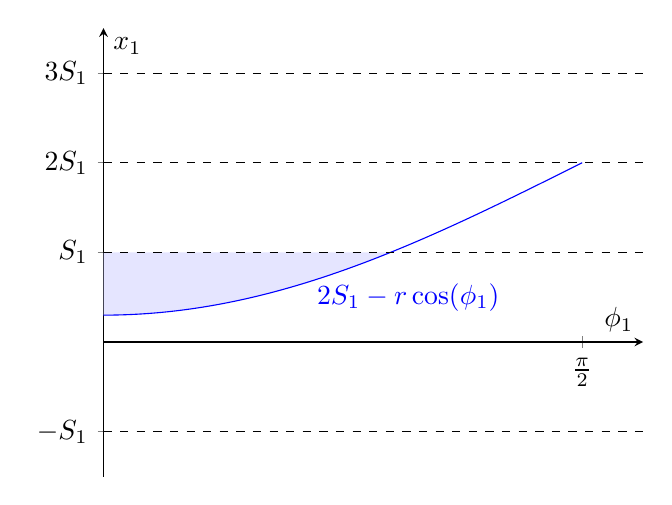
\begin{tikzpicture}
        \begin{axis}[
            axis lines=middle,
            xlabel={$\phi_1$},
            ylabel={$x_1$},
            xmin=0, xmax=pi/2+0.2, % Adjust the x-axis limits
            ymin=-1.5, ymax=3.5, % Adjust the y-axis limits
            xtick={0,pi/2}, % Adjust the x-axis tick positions
            ytick={-1,0,1,2,3}, % Adjust the y-axis tick positions
            xticklabels={0, $\frac{\pi}{2}$}, % Adjust the x-axis tick labels
			yticklabels={$-S_1$, 0, $S_1$, $2S_1$, $3S_1$}
        ]

			% Parameters
			\def\S{1} % Replace with your desired value for S
			\def\r{1.7} % Replace with your desired value for r
			\def\c{2}
			\pgfmathsetmacro\endshaded{acos(\S*(\c-1)/\r)}


			% Plot the function
			\addplot[blue, domain=0:pi/2, samples=100, name path=curve] {\S*\c - \r*cos(deg(x))};

			% Label the function
			\node[blue] at (axis cs:1,.5) {$2S_1 - r\cos(\phi_1)$};

			% Add dashed lines at -S, S, 2S, and 3S on the y-axis
			\draw[dashed] (axis cs:0,-\S) -- (axis cs:pi/2+0.2,-\S);
			\draw[dashed, name path = Sline] (axis cs:0,\S) -- (axis cs:pi/2+0.2,\S);
			\draw[dashed] (axis cs:0,2*\S) -- (axis cs:pi/2+0.2,2*\S);
			\draw[dashed] (axis cs:0,3*\S) -- (axis cs:pi/2+0.2,3*\S);

			\addplot[blue!20, fill opacity=0.5] fill between[of=curve and Sline, soft clip={domain=0:0.942}];

        \end{axis}
    \end{tikzpicture}
    \caption{Domain of integration when $r<S_1c$}\label{fig:short r int}
\end{figure}

\begin{figure} 
	\centering
    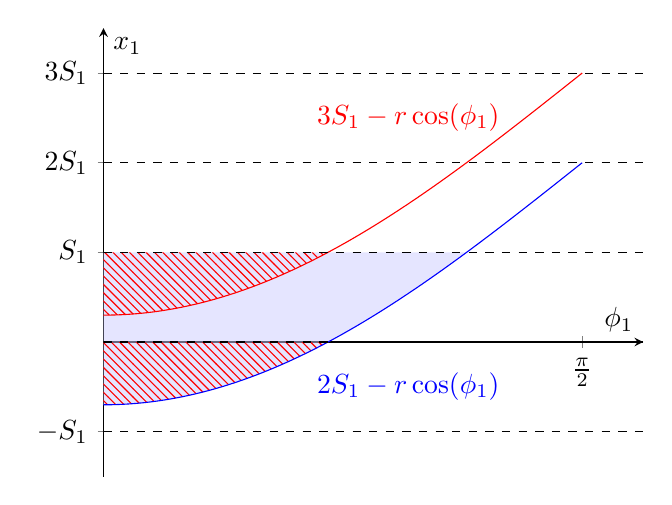
\begin{tikzpicture}
        \begin{axis}[
            axis lines=middle,
            xlabel={$\phi_1$},
            ylabel={$x_1$},
            xmin=0, xmax=pi/2+0.2, % Adjust the x-axis limits
            ymin=-1.5, ymax=3.5, % Adjust the y-axis limits
            xtick={0,pi/2}, % Adjust the x-axis tick positions
            ytick={-1,0,1,2,3}, % Adjust the y-axis tick positions
            xticklabels={0, $\frac{\pi}{2}$}, % Adjust the x-axis tick labels
			yticklabels={$-S_1$, 0, $S_1$, $2S_1$, $3S_1$}
        ]

			% Parameters
			\def\S{1} % Replace with your desired value for S
			\def\r{2.7} % Replace with your desired value for r
			\def\c{2}
			\pgfmathsetmacro\endshaded{acos(\S*(\c-1)/\r)}


			% Plot the function
			\addplot[blue, domain=0:pi/2, samples=100, name path=curve] {\S*\c - \r*cos(deg(x))};
			\addplot[red, domain=0:pi/2, samples=100, name path=Hcurve] {\S*(\c+1) - \r*cos(deg(x))};

			% Label the function
			\node[blue] at (axis cs:1,-.5) {$2S_1 - r\cos(\phi_1)$};
			\node[red] at (axis cs:1,2.5) {$3S_1 - r\cos(\phi_1)$};

			% Add dashed lines at -S, S, 2S, and 3S on the y-axis
			\draw[dashed] (axis cs:0,-\S) -- (axis cs:pi/2+0.2,-\S);
			\draw[dashed, name path = oline] (axis cs:0,0) -- (axis cs:pi/2+0.2,0);
			\draw[dashed, name path = Sline] (axis cs:0,\S) -- (axis cs:pi/2+0.2,\S);
			\draw[dashed] (axis cs:0,2*\S) -- (axis cs:pi/2+0.2,2*\S);
			\draw[dashed] (axis cs:0,3*\S) -- (axis cs:pi/2+0.2,3*\S);

			\addplot[blue!20, fill opacity=0.5] fill between[of=curve and Sline, soft clip={domain=0:1.191}];
			\addplot[red!20, pattern=north west lines, pattern color=red] fill between[of=Hcurve and Sline, soft clip={domain=0:0.736}];
			\addplot[red!20, pattern=north west lines, pattern color=red] fill between[of=curve and oline, soft clip={domain=0:0.736}];

        \end{axis}
    \end{tikzpicture}
    \caption{}\label{fig:long r int}
\end{figure}

When $r$ exceeds the value of $S_1c$, the region enclosed by the curve exceeds the domain of
interest. Specifically, the region where $x_1<0$. One way to correct for this is to realize
that the area between the curve and the axis is identical to the area between $x_1=S_1$ and
the same curve translated up by $S_1$. This is convenient as we have an expression for the
integrals in the region between curves of the form $S_1c-rcos\phi_1$ and $S_1$. Because the integrand is invariant to
changes in $x_1$, we can guarantee that the integrals evaluate to the same value. 

As such, the result is simply
\begin{align}
	P_1(c | r>S_1c) &= \frac{2r}{S_1 B(\frac{D-1}{2}, \frac{1}{2})} (\xi(c) - \xi(c+1)) \\
	&= P_1(c | r<S_1c) - P_1(c+1 | r<S_1c)
\end{align}


\subsection{Numeric Validation of Crossing $N=1$}
To summarize, the probability that a randomly placed line segment will cross at least $c$
hyperplanes given that there is 1 set of parallel hyperplanes with spacing $S_1$ is as follows

\begin{gather}
	P(C\ge c | r, D, N=1, S) = \begin{cases}
		0 & r < S(c-1) \\ 
		\cfrac{2r}{S_1 B(\frac{D-1}{2}, \frac{1}{2})} \xi(c)  & S_1 (c-1) < r < S_1 c \\
		\cfrac{2r}{S_1 B(\frac{D-1}{2}, \frac{1}{2})} (\xi(c)-\xi(c+1)) & r > S_1c		
	\end{cases} \\
	\xi(c) = \frac{-\gamma}{2}B\left(\frac{D-1}{2}, \frac{1}{2}\right)\left(g(\gamma, D-2)-\gamma(1-\gamma^2)^{(D-1)/2}\sum_{k=1}^{\lfloor \frac{D-2}{2} \rfloor}\frac{B(\frac{D-2k}{2}, \frac{1}{2})}{\pi(1-\gamma^2)^k}\right) + \frac{1}{D-1}(1-\gamma^2)^{(D-1)/2} \\
	\gamma = \frac{S_1(c-1)}{r} 
\end{gather}

To compare this against numeric simulation, we must generate many samples with uniform spherical
distribution. We use the method proposed by Marsaglia of normalizing rotationally symmetric
distribution (such as a D-dimensional gaussian variable).

\begin{figure}[h]
	\centerline{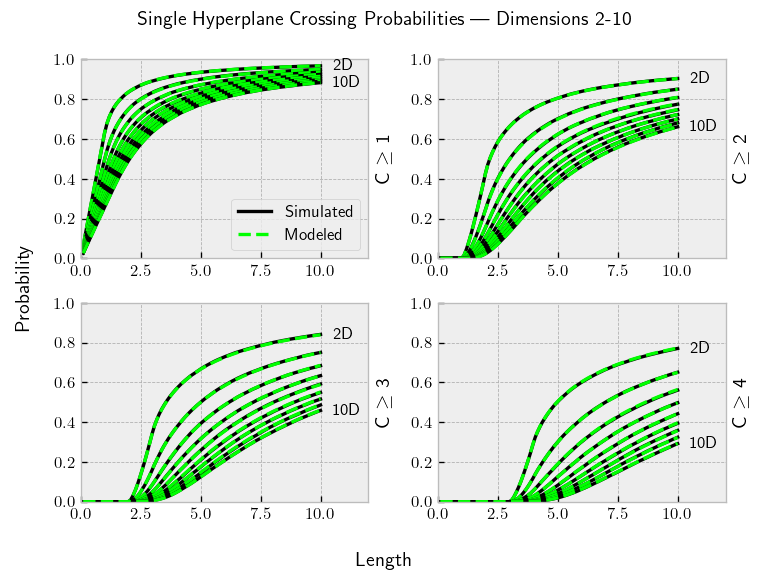
\includegraphics[width=5in]{numeric_sim_N1.png}}
	\caption{Comparison of numerically simulated crossing probability and modeled probabilities
	for $c\in[1, 2, 3, 4]$. A hyperplane spacing of 1 is used. Solutions are shown for dimensions 2 through 10. 10,000 samples were
	used in the numeric simulation.}
	\label{fig:numeric sim N1}
\end{figure}

\section{Probability of crossing $N\ge 1$}
When there is only a single set of parallel hyperplanes, there is only one way for a needle to make
$c$ intersections. The needle would have to go through $c$ hyperplanes in a single direction.
When we increase the number of orthogonal sets of hyperplanes then we must deal with the fact that
there are now many ways to cross $c$ hyperplanes due to the many combinations of directions available.

For instance, if $N=2$ and we want to know when $C=2$, then a valid number of crossings occurs if the
needle crosses 2 hyperplanes in $x_1$ and 0 in $x_2$, or 1 hyperplane in each direction, or 0 hyperplanes
in $x_1$ and 2 in $x_2$.

For simplicity, we begin with the assumption that $r<\min(S)$ to ensure that the needle can never cross
more than 1 hyperplane in any given direction. We will then investigate what happens as $r$ grows in
size.

\subsection{$N\ge 1, r<\min(S)$}
Let $P_{1\cap2\cap\hdots\cap n}(C=n|r,D,N,S)=P_{1\cap\hdots\cap n}$ be the probability that the
needle crosses at least 1 hyperplane in each of the directions $x_1, x_2, \hdots, x_n$. Similarly,
let $P_{1\cup2\cup\hdots\cup n}(C\ge 1|r,D,N,S)=P_{1\cup\hdots\cup n}(1)$ be the probability that
the needle crosses at least 1 hyperplane in direction $x_1$ or $x_2$ or so on. This probability
is equivalent to the probability that $P(C\ge 1|r,D,N,S)$ as crossing a hyperplane in any 
direction is sufficient to meet the condition $C\ge 1$. Using the inclusion-exclusion principle,
this probability can be written as the following sum.

\begin{equation}
	P(C\ge 1|r, D, N, S) = P_{1\cup2\cup\hdots\cup N} = \sum_{k=1}^N (-1)^{k+1}\left(\sum_{1\le i_1 < \hdots < i_k \le N}P_{i_1 \cap \hdots \cap i_k} \right)
\end{equation}

Similarly, for $C\ge c$, we can define the set of events $E_c^N$ which consists of each of the
$N \choose c$ hyperplane crossing combinations. For example, $E_2^3=\{(1,2), (1,3), (2,3)\}$.
If the needle crosses hyperplanes in all of the directions listed in any element of $E_c^N$,
then the crossing condition for the criteria $C \ge c$ has been met.

\begin{equation}
	P(C\ge c|r, D, N, S) = P_{(\cap E_c^N[1])\cup(\cap E_c^N[2])\cup\hdots\cup(\cap E_c^N[{N \choose c}])} = \sum_{k=1}^N (-1)^{k+1}\left(\sum_{1\le i_1 < \hdots < i_k \le N}P_{E_c^N[i_1] \cap \hdots \cap E_c^N[i_k]} \right)
\end{equation}

This expression requires an equation for the probability of having at least 1 crossing in
multiple hyperplane directions. 

\begin{proposition}
	For any given set of hyperplane directions, $\emph{H}$, the probability that a needle would cross
	at least 1 hyperplane in each of the specified directions can be represented as follows.
	\begin{equation}
		P_{H_1 \cap \hdots \cap H_N} = \frac{r^N \Gamma(\frac{D}{2})}{(\prod_{i=1}^N S_i) \pi^{N/2} \Gamma(\frac{D+N}{2})}
	\end{equation}
\end{proposition}

\begin{proof}
	
\end{proof}

%Below here is template stuff ==========================================================
\section{Headings: first level}
\label{sec:headings}

\lipsum[4] See Section \ref{sec:headings}.

\subsection{Headings: second level}
\lipsum[5]
\begin{equation} 
	\xi _{ij}(t)=P(x_{t}=i,x_{t+1}=j|y,v,w;\theta)= {\frac {\alpha _{i}(t)a^{w_t}_{ij}\beta _{j}(t+1)b^{v_{t+1}}_{j}(y_{t+1})}{\sum _{i=1}^{N} \sum _{j=1}^{N} \alpha _{i}(t)a^{w_t}_{ij}\beta _{j}(t+1)b^{v_{t+1}}_{j}(y_{t+1})}}
\end{equation}



\subsubsection{Headings: third level}
\lipsum[6]

\paragraph{Paragraph}
\lipsum[7]



\section{Examples of citations, figures, tables, references}
\label{sec:others}

\subsection{Citations}
Citations use \verb+natbib+. The documentation may be found at
\begin{center}
	\url{http://mirrors.ctan.org/macros/latex/contrib/natbib/natnotes.pdf}
\end{center}

Here is an example usage of the two main commands (\verb+citet+ and \verb+citep+): Some people thought a thing \citep{kour2014real, hadash2018estimate} but other people thought something else \citep{kour2014fast}. Many people have speculated that if we knew exactly why \citet{kour2014fast} thought this\dots

\subsection{Figures}
\lipsum[10]
See Figure \ref{fig:fig1}. Here is how you add footnotes. \footnote{Sample of the first footnote.}
\lipsum[11]

\begin{figure}
	\centering
	\fbox{\rule[-.5cm]{4cm}{4cm} \rule[-.5cm]{4cm}{0cm}}
	\caption{Sample figure caption.}
	\label{fig:fig1}
\end{figure}

\subsection{Tables}
See awesome Table~\ref{tab:table}.

The documentation for \verb+booktabs+ (`Publication quality tables in LaTeX') is available from:
\begin{center}
	\url{https://www.ctan.org/pkg/booktabs}
\end{center}


\begin{table}
	\caption{Sample table title}
	\centering
	\begin{tabular}{lll}
		\toprule
		\multicolumn{2}{c}{Part}                   \\
		\cmidrule(r){1-2}
		Name     & Description     & Size ($\mu$m) \\
		\midrule
		Dendrite & Input terminal  & $\sim$100     \\
		Axon     & Output terminal & $\sim$10      \\
		Soma     & Cell body       & up to $10^6$  \\
		\bottomrule
	\end{tabular}
	\label{tab:table}
\end{table}

\subsection{Lists}
\begin{itemize}
	\item Lorem ipsum dolor sit amet
	\item consectetur adipiscing elit.
	\item Aliquam dignissim blandit est, in dictum tortor gravida eget. In ac rutrum magna.
\end{itemize}


\bibliographystyle{unsrtnat}
\bibliography{references}  %%% Uncomment this line and comment out the ``thebibliography'' section below to use the external .bib file (using bibtex) .


%%% Uncomment this section and comment out the \bibliography{references} line above to use inline references.
% \begin{thebibliography}{1}

% 	\bibitem{kour2014real}
% 	George Kour and Raid Saabne.
% 	\newblock Real-time segmentation of on-line handwritten arabic script.
% 	\newblock In {\em Frontiers in Handwriting Recognition (ICFHR), 2014 14th
% 			International Conference on}, pages 417--422. IEEE, 2014.

% 	\bibitem{kour2014fast}
% 	George Kour and Raid Saabne.
% 	\newblock Fast classification of handwritten on-line arabic characters.
% 	\newblock In {\em Soft Computing and Pattern Recognition (SoCPaR), 2014 6th
% 			International Conference of}, pages 312--318. IEEE, 2014.

% 	\bibitem{hadash2018estimate}
% 	Guy Hadash, Einat Kermany, Boaz Carmeli, Ofer Lavi, George Kour, and Alon
% 	Jacovi.
% 	\newblock Estimate and replace: A novel approach to integrating deep neural
% 	networks with existing applications.
% 	\newblock {\em arXiv preprint arXiv:1804.09028}, 2018.

% \end{thebibliography}


\end{document}
